\section{Redes definidas por software}
\label{sec:sdn-openflow}

As redes de computadores se tornaram parte da infraestrutura crítica de empresas, escolas e residências, tendo crescido bastante desde a sua origem. O sucesso das redes de computadores se deve, em grande parte, à simplicidade de seu núcleo. Na arquitetura atual, a inteligência está localizada nos sistemas de borda, enquanto que o núcleo é simples e transparente. Embora essa simplicidade tenha tido sucesso, também é razão para o seu engessamento, pois apresenta limitações estruturais que são difíceis de serem resolvidas, tais como escalabilidade, mobilidade e gerenciamento de serviço \cite{Clarkl:2004}.

Por causa desta expansão, o trabalho dos pesquisadores da área tornou-se muito mais importante, porém mesmo com o grande número de equipamentos e protocolos criados para suportar essa expansão, surgiu uma enorme barreira: a maioria das ideias que surgem não conseguem ser testadas por falta de maneiras práticas que possibilitem a realização de experimentos com novos protocolos em uma rede realista, para que possa obter a confiança necessária para uma implantação em escala global \cite{McKeown:2008}. 

Como apresentado por Kreutz \textit{et al.} (2014)\nocite{Kreutz:2014}, redes de computadores podem ser separadas em três planos: de controle, de dados e de gerência. 

Entende-se por plano de controle a porção da rede que abriga os \textit{softwares} responsáveis por ditar o comportamento da rede. Decisões de roteamento, \textit{firewall}, priorização de pacotes são de responsabilidade do plano de controle. O plano de dados é o que executa o encaminhamento dos pacotes com base nas regras ditadas pelo plano de controle. Já o plano de gerência inclui serviços utilizados para monitorar a rede e configurar remotamente o plano de controle utilizando protocolos como \gls{snmp} \cite{RFC1157}. 

Em síntese, o plano de gerência define as regras da rede, o de controle implementa essas regras e o plano de dados realiza o encaminhamento de pacotes de acordo com as regras impostas pelo plano de controle. Em redes \gls{ip} tradicionais, os planos de controle e dados são acoplados em um mesmo hardware, tornando a arquitetura de rede complexa e por consequência dificulta a sua configuração e o seu gerenciamento.

Para tentar contornar esse problema, a comunidade de pesquisa em redes de computadores tem investido em iniciativas que levem a implantação de redes com maiores recursos de programação, de forma que novas tecnologias possam ser inseridas na rede de forma gradual. Exemplos de iniciativas desse tipo são as propostas de redes ativas (\textit{active networks}) \cite{Tennenhouse:1997}, de \textit{testbeds} como o PlanetLab \cite{Chun:2003}, GENI \cite{Turner:2006} e, mais recentemente o FIBRE \cite{Salmito:2014}. Redes ativas, tiveram pouca aceitação pela necessidade de alteração dos elementos de rede para permitir que se tornassem programáveis. Iniciativas mais recentes como PlanetLab, GENI e FIBRE, apostam na adoção de recursos de virtualização para facilitar a transição para novas tecnologias. Apesar de serem consideradas de grande potencial a longo prazo, tais iniciativas ainda enfrentam desafios como garantir o desempenho exigido pelas aplicações utilizadas hoje utilizando-se tais elementos virtualizados \cite{Guedes:2006}.

Uma outra forma de abordar esse problema, consiste em estender o \textit{hardware} de encaminhamento de pacotes de forma mais restrita. Considerando-se que a operação que necessita de alto desempenho nos elementos de comutação é o encaminhamento de pacotes (plano de dados), algumas iniciativas propõem manter essa operação pouco alterada, para manter a viabilidade de desenvolvimento de hardware de alto desempenho, mas com uma possibilidade de maior controle por parte do administrador da rede. 

\gls{sdn} introduz uma perspectiva flexível para programar e manter a operacionalidade da rede  buscando desacoplar os planos de dados e de controle, desta forma, tira-se a autonomia dos equipamentos de rede que se tornam apenas encaminhadores de pacotes. Já a lógica de controle é movida para uma entidade externa, centralizada, implementada em \textit{software}. Esta, chamada de controlador, tem por funcionalidade prover a lógica de funcionamento da rede o que torna o desenvolvimento de serviços mais facilmente implementáveis, já que não há a necessidade de implementação em cada dispositivo. 

No plano de dados, o encaminhamento de pacotes, que antes era baseado em destino, passa a ser por fluxo que é definido pela combinação de campos das camadas de enlace, de rede ou de transporte, segundo o modelo TCP/IP. Dessa forma mantém-se o alto desempenho no encaminhamento de pacotes em \textit{hardware}, aliado à flexibilidade de se implementar aplicações em \textit{software}, utilizando protocolo aberto para programação da lógica do equipamento que é abstraída dos dispositivos de encaminhamento \cite{Kim:2013, Tootoonchian:2010, Rothenberg:2010}.

Pensando nisso, nasceu o OpenFlow \cite{McKeown:2008}, que por sua vez, deu origem ao conceito de \textit{Software Defined Networking}, ou redes definidas por software. A Figura \ref{fig:arch-old-sdn} apresenta um comparativo entre o modelo tradicional de rede, onde onde ambos os planos, de controle e de dados, são localizados em um mesmo dispositivo e o modelo \gls{sdn} que possui controle centralizado e apenas o plano de dados no dispositivo comutador.

\begin{figure}[H]
  \centering
  \caption{Modelos de rede tradicional e SDN}
  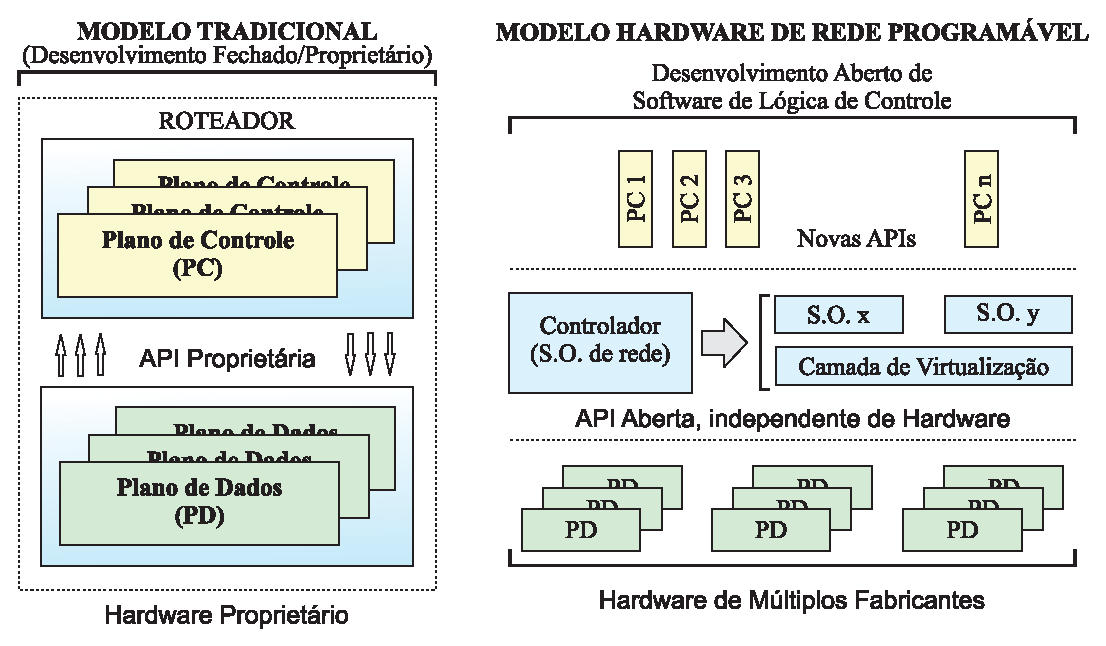
\includegraphics[width=.80\textwidth]{images/arch-old-sdn.eps}
  \fonte{Rothenberg \textit{et al.} (2010) \nocite{Rothenberg:2010}}
  \label{fig:arch-old-sdn}
\end{figure}
\FloatBarrier

O protocolo OpenFlow é implementado em ambos os planos e dispõe de um protocolo de comunicação entre o controlador e \textit{switches}. Para garantir a confiabilidade dessa comunicação é recomendada a utilização do protocolo \gls{ssl} \cite{RFC6101} porém algumas alternativas incluem \gls{tcp}, utilizadas especialmente em redes virtuais devido à sua simplicidade, pois não necessitam de chaves criptográficas \cite{Rothenberg:2010}.

OpenFlow explora a existência de tabelas de fluxo (\textit{flow tables}) em dispositivos \textit{Ethernet} modernos. Essas tabelas são alimentadas em tempo de execução e utilizadas para implementar \textit{firewalls} \cite{Oppliger:1997}, \gls{nat} \cite{RFC3022}, \gls{qos} \cite{Aurrecoechea:1998} e coleta de estatísticas. Normalmente são proprietárias mas há um conjunto de funções que são comuns na maioria dos dispositivos. Com isso, uma forma padrão de manipulação das tabelas de fluxo pode ser implementada, independente de fornecedor. Desta maneira, OpenFlow fornece um padrão para manipulação das tabelas de fluxo, permitindo assim a partição do tráfego, o agrupamento ou isolamento da rede e o processamento ou controle do fluxo de dados, da forma desejada com base no fluxo \cite{Kontesidou:2009}.

Os principais componentes de uma arquitetura \gls{sdn} são:
\begin{itemize}
    \item Comutadores (\textit{switches}) \textit{OpenFlow};
    \item Controlador; e
    \item Protocolo de comunicação.
\end{itemize}
Estes componentes podem fazer uso do protocolo OpenFlow e/ou de outros protocolos. Por ser o primeiro e também o mais utilizado, o protocolo OpenFlow é utilizado neste trabalho como padrão de comunicação entre os dispositivos.

%=====================================================================

\subsection{Comutadores}
\label{subsec:comutador}

É o elemento responsável pelo encaminhamento dos pacotes pela rede. Pode ser específico para OpenFlow, ou ter suporte ao mesmo. No comutador (\textit{switch}) OpenFlow é mantida uma tabela de fluxo (\textit{flow table}) que armazena informações sobre como os pacotes serão processados, estatísticas, prioridades e tempo limite para novos fluxos. Além disso, cada regra é composta por um conjunto de campos do cabeçalho do pacote que podem ser visualizadas na Figura \ref{fig:flow-table}, assim como as informações de ações e estatísticas.

\begin{figure}[H]
  \centering
  \caption{Tabela de fluxo}
  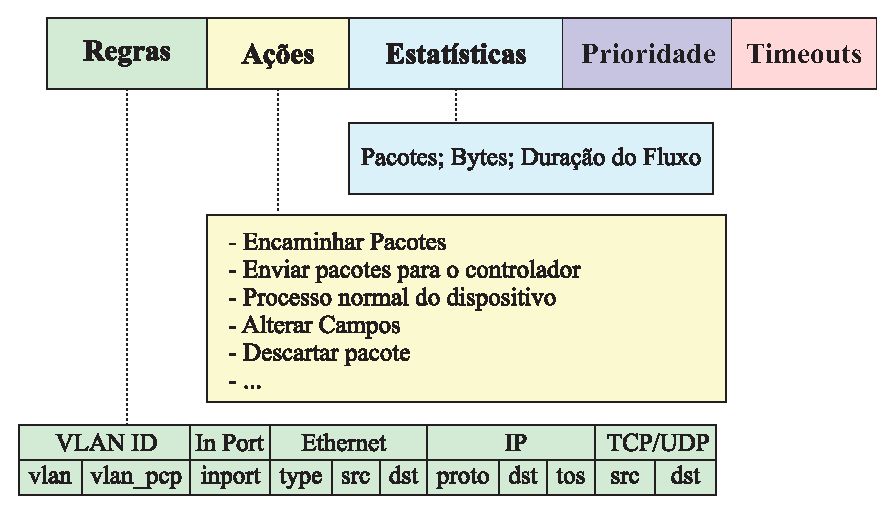
\includegraphics[width=.65\textwidth]{images/flow-table.eps}
  \label{fig:flow-table}
  \fonte{Adaptado de Costa (2014) \nocite{Costa:2004}}
\end{figure}
\FloatBarrier
%Copiado e artigo 6, reescrever
Quando um pacote chega a um equipamento com OpenFlow habilitado, os cabeçalhos do pacote são comparados (\textit{match}) às regras das entradas das tabelas de fluxos, os contadores são atualizados e as ações correspondentes são realizadas. Se não houver correspondência  (\textit{table miss}) entre o pacote e alguma entrada da tabela de fluxos, o pacote é encaminhado, por completo, ao controlador. Alternativamente, apenas o cabeçalho é encaminhado ao controlador mantendo o pacote armazenado no \textit{buffer} do \textit{hardware}. A Figura \ref{fig:fluxo-tmp} ilustra, através de um diagrama simplificado, o tratamento recebido por pacotes em um \textit{switch} OpenFlow.

Os pacotes que chegam ao controlador normalmente correspondem ao primeiro pacote de um novo fluxo ou, em função do tipo de pacote e da aplicação, o controlador pode decidir por instalar uma regra no \textit{switch} para que todos os pacotes de determinado fluxo sejam enviados para o controlador para serem tratados individualmente. Esse último caso corresponde, em geral, a pacotes de controle  (\gls{icmp} \cite{RFC0792}, \gls{dns} \cite{RFC7719}, \gls{dhcp} \cite{RFC2131}) ou de protocolos de roteamento (\gls{ospf} \cite{RFC2328}, \gls{bgp} \cite{RFC4271}).
Todos os pacotes de uma mesma faixa de endereços \gls{ip}, ou uma conexão \gls{tcp} em determinada porta são considerados fluxos.

\begin{figure}[H]
  \centering
  \caption{Diagrama simplificado do tratamento de um pacote no \textit{switch} OpenFlow}
  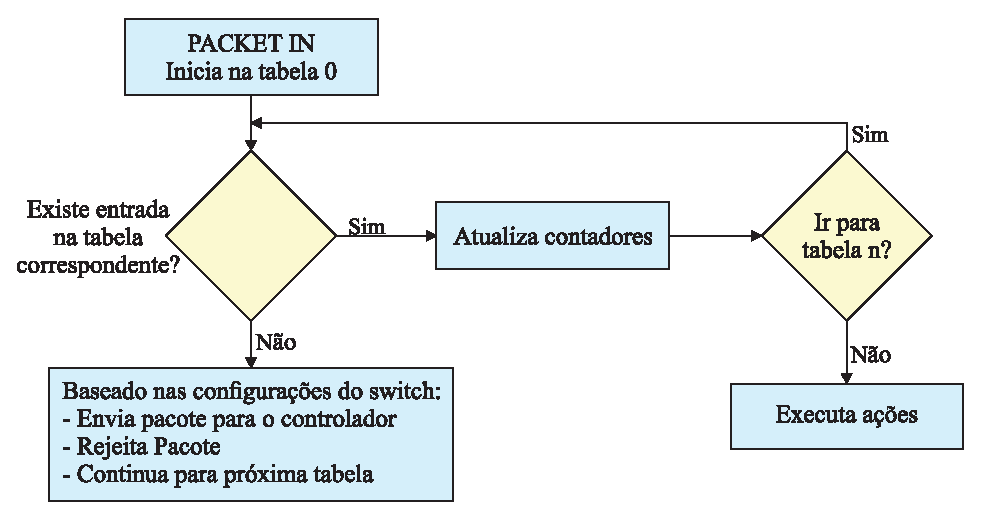
\includegraphics[width=.80\textwidth]{images/flow.eps}
  \label{fig:fluxo-tmp}
  \fonte{Elaborado pelo autor a partir da especificação OpenFlow\\\cite{OpenFlowSpec:2014}}
\end{figure}
\FloatBarrier

A cada pacote recebido, é realizada a atualização dos contadores na tabela de fluxo.
Esses contadores são usados para geração de estatísticas, de maneira a monitorar o número de pacotes e bytes de cada fluxo, além do tempo de duração desde o seu início. O Quadro \ref{tab:contadores} apresenta alguns dos contadores disponíveis na tabela de fluxo. Com o auxílio deste podem ser implementados recursos de monitoramento e segurança do tráfego na rede.

\begin{table}[H]
  \centering
  %\captionof{figure}[tab:contadores]{Contadores da tabela de fluxo}
  \caption{Contadores da tabela de encaminhamento}
  \begin{tabular}{|l|c|} \hline
	\textbf{Contator} & \textbf{Tamanho em bits} \\ \hline
	\multicolumn{2}{|c|}{Por Tabela} \\ \hline
	Número de entradas Ativas & 32 \\ \hline
	Número de pacotes pesquisados & 64 \\ \hline
	Número de pacotes encontrados na tabela & 64 \\ \hline
	\multicolumn{2}{|c|}{Por fluxo} \\ \hline
	Número de pacotes recebidos & 64 \\ \hline
	Número de bytes recebidos & 64 \\ \hline
	Duração (segundos) & 32 \\ \hline
	Duração (nano segundos) & 32 \\ \hline
	\multicolumn{2}{|c|}{Por porta} \\ \hline
	Número de pacotes recebidos & 64 \\ \hline
	Número de pacotes transmitidos & 64 \\ \hline
	Número de bytes recebidos & 64 \\ \hline
	Número de bytes transmitidos & 64 \\ \hline
	Número de pacotes perdidos no recebimento & 64 \\ \hline
	Número de pacotes perdidos na transmissão & 64 \\ \hline
	Número de erros recebidos & 64 \\ \hline
  \end{tabular}
  \label{tab:contadores}
  \fonte{Elaborado pelo autor a partir da especificação OpenFlow\\  \cite{OpenFlowSpec:2014}}
\end{table}

Neste projeto o comutador a ser utilizado é o Open vSwitch \cite{website:ovs}, um \textit{switch} virtual com suporte a OpenFlow. Este comutador é projetado para permitir a automatização de grandes redes através da extensão programática, suportando ainda interfaces e protocolos de gerenciamento como, por exemplo, NetFlow \cite{rfc3954}, sFlow \cite{rfc3176} e IPFIX \cite{rfc5153}. Além disso, pode suportar a distribuição através de múltiplos servidores físicos \cite{website:ovs}.
%=====================================================================

\subsection{Controlador}
\label{subsec:controlador}

O controlador, como já citado, é o \textit{software} responsável por tomar decisões e adicionar e remover as entradas na tabela de encaminhamento, de acordo com o objetivo desejado. Exerce a função de uma camada de abstração da infraestrutura física, facilitando a criação de aplicações e serviços que gerenciem as entradas de fluxos na rede. Esse modelo assemelha-se a outros sistemas de \textit{software} que proveem abstração do \textit{hardware} e funcionalidade reutilizável. Dessa forma, o controlador atua como um \gls{so} para gerenciamento e controle das redes, e oferece uma plataforma com base na reutilização de componentes e na definição de níveis de abstração. Contudo, novas aplicações de rede podem ser desenvolvidas rapidamente \cite{Gude:2008}.

O controlador fornece uma interface para criar, modificar e controlar o fluxo de tabelas do comutador. É executado normalmente em um servidor conectado à rede e pode ser um para todos os comutadores da rede, um para cada comutador ou um para um conjunto de comutadores.  Portanto, a funcionalidade da rede de controle pode ser completamente ou localmente centralizada de acordo de como o gerenciamento dos comutadores é realizada. A exigência, no entanto, é que, se houver mais do que um controlador de processos, eles devem ter a mesma visão da topologia da rede, em qualquer momento dado. A visão de rede inclui a topologia a nível de \textit{switch}, as localizações dos usuários, \textit{hosts}, \textit{middleboxes} e outros elementos de rede e serviços. Além disso inclui todas as ligações entre os nomes e endereços.

O controlador é parte integrante de uma arquitetura de rede \gls{sdn} e para que sua comunicação com \textit{switches} OpenFlow ocorra, o controlador deve ter suporte ao mesmo. Atualmente, existem várias implementações controlador disponíveis que implementam o protocolo OpenFlow, entre os principais não comerciais estão \cite{Kreutz:2013,Xia:2015}:

\begin{itemize}
    \item \textbf{NOX} - Desenvolvido em C++, foi o primeiro controlador OpenFlow \cite{Gude:2008}. Porém não foi fortemente utilizado por causa de deficiências na sua implementação e na documentação.
    \item \textbf{POX} - Sucessor do NOX, foi desenvolvido como uma alternativa mais amigável e tem sido implementado por um grande número de engenheiros e programadores \gls{sdn}. Comparando com NOX, POX tem um ambiente de desenvolvimento mais fácil de trabalhar com uma API razoavelmente bem escrita e documentada. Também fornece uma interface Web e é escrito em Python \cite{website:pox}.
    \item \textbf{Beacon} - É um controlador SDN bem escrito e organizado. Escrito em Java, Beacon foi o primeiro controlador com o qual iniciantes pudessem trabalhar e criar um ambiente \gls{sdn}, no entanto, era limitado à topologias de rede estrela \cite{Erickson:2013}.
    \item \textbf{Floodlight} - Uma ramificação do Beacon. Enquanto que seu início tenha sido baseado no Beacon este foi desenvolvido utilizando Apache Ant, uma ferramenta popular para compilação e construção de \textit{software}, o que tornou o desenvolvimento do Floodlight mais fácil e flexível. Floodlight possui uma comunidade ativa e um grande número de recursos que podem ser adicionados ao sistema. Possui interface baseada em java e baseada em Web, além de possuir uma Interface de Programação de Aplicações (\gls{api}) \gls{rest} ou, em português, Transferência de Estado Representacional \cite{website:floodlight}.
    \item \textbf{OpenDayLight} - É um projeto colaborativo da Linux Fundation e tem sido altamente suportado por empresas como Cisco e Big Switch. Desenvolvido em Java, também inclui \gls{api} \gls{rest} e interface web. Possui suporte à \gls{sdn}, \gls{nv} , ou Virtualização de redes \cite{Chowdhury:2009} e \gls{nfv}, ou Virtualização da Funções da Rede \cite{Hawilo:2014}. Além disso, possui um grande número de módulos que podem ser utilizados para atender aos requisitos de uma organização \cite{website:odl}.
    \item \textbf{Ryu NOS} - É um \textit{framework} de \gls{sdn} baseado em componentes. O Ryu fornece componentes de software com \glspl{api} bem definidas que tornam mais fácil para os desenvolvedores criar novas aplicações de gerenciamento e controle de rede. O Ryu suporta vários protocolos para gerenciar dispositivos de rede, como OpenFlow, Netconf, OF-config, etc. Sobre o OpenFlow, o Ryu suporta totalmente as extensões 1.0, 1.2, 1.3, 1.4, 1.5 e Nicira. Todo o código está disponível gratuitamente sob a licença Apache 2.0 \cite{website:ryu}.
\end{itemize}

%=====================================================================

\subsection{Protocolo OpenFlow}
\label{subsec:protocolo-comunicacao}

O protocolo de comunicação entre os dois planos é realizado por três tipos de mensagens: controlador para o \textit{switch}, assíncrona e simétricas. 

Mensagens do tipo controlador para \textit{switch} são mensagens que o controlador envia para obter informações sobre o estado do \textit{switch}, como por exemplo verificar estatísticas de um determinado fluxo \cite{OpenFlowSpec:2014}. Essas mensagens podem ser:
%Rescrever
\begin{itemize}
    \item \textit{\textbf{Features}}: ao estabelecer uma conexão, o controlador envia esta mensagem requisitando que o \textit{switch} informe suas capacidades.
    \item \textit{\textbf{Configuration}}: o controlador envia parâmetros de configuração para os \textit{switches}. 
    \item \textit{\textbf{Modify-State}}: utilizado pelo controlador para gerenciar o estado dos \textit{switches}, deletar ou modificar regras na tabela de fluxos.
    \item \textit{\textbf{Read-State}}: utilizado pelo controlador para coletar estatísticas das tabelas de fluxos do \textit{switch}.
    \item \textit{\textbf{Packet-Out}}: utilizada pelo controlador para enviar pacotes por uma porta específica.
    \item \textit{\textbf{Barrier}}: utilizada para verificar se as dependências das mensagens foram alcançadas ou receber notificação sobre tarefas concluídas.
     \item \textit{\textbf{Role Request}}: mensagens usadas pelo controlador para configurar seu canal OpenFlow.
\end{itemize}

Mensagens assíncronas são enviadas pelo \textit{switch} sem a solicitação do controlador. \textit{Switches} enviam mensagens assíncronas para os controladores para denotar uma chegada de pacotes ou mudança de estado \cite{OpenFlowSpec:2014}. Os principais tipos de mensagens assíncronas são descritas abaixo.
\begin{itemize}
    \item \textit{\textbf{Packet-In}}: enviado pelo \textit{switch} quando há uma ação explícita na tabela de fluxos para que seja enviado para o controlador ou quando não há um \textit{match} para o pacote.
    \item \textit{\textbf{Flow-Removed}}: informa o controlador sobre a remoção de regras no \textit{switch}.
    \item \textit{\textbf{Port Status}}: obtém status das portas do \textit{switch}.
    \item \textit{\textbf{Role Status}}: \textit{switch} informa o controlador sobre a alterações em suas regras.
    \item \textit{\textbf{Controller Status}}: \textit{switch} informa o controlador sobre a mudança em um canal OpenFlow.
    \item \textit{\textbf{Flow-monitor}}: informa o controlador sobre uma mudança na tabela de fluxo.
\end{itemize}

Finalmente, mensagens simétricas são iniciadas tanto pelo controlador como pelo \textit{switch} sem nenhuma solicitação, por exemplo o início de conexão entre controlador e \textit{switch} \cite{OpenFlowSpec:2014}. Essas mensagens são:
\begin{itemize}
    \item \textit{\textbf{Hello}}: esta mensagem é utilizada no início da conexão entre \textit{switch} e controlador.
    \item \textit{\textbf{Echo}}: utilizado para obter informações sobre a conexão entre \textit{switch} e controlador como:
latência, largura de banda e conectividade.
    \item \textit{\textbf{Error}}:  o \textit{switch} pode enviar mensagens para notificar problemas ao controlador por mensagens de erro.
    \item \textit{\textbf{Experimenter}}: na versão 1.5.0 do protocolo OpenFlow, esta mensagem é utilizada para adicionar funcionalidades experimentais.
\end{itemize}

Cada mensagem é enviada encapsulada em um pacote definido pelo protocolo OpenFlow e que é representado na Figura \ref{fig:openflow-message} abaixo.

\begin{figure}[H]
  \centering
  \caption{Formato da mensagem OpenFlow}
  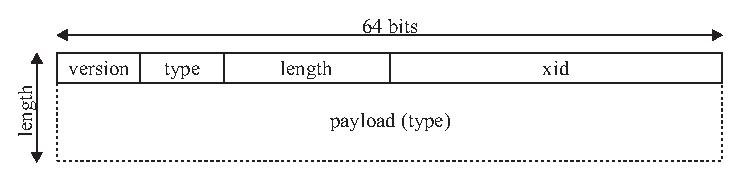
\includegraphics[width=.80\textwidth]{images/openflow-message.eps}
  \label{fig:openflow-message}
  \fonte{\centering
  Elaborado pelo autor a partir de informações da especificação OpenFlow.}
\end{figure}
\FloatBarrier

O campo \textit{version} indica a versão do protocolo que está sendo utilizada. Já o  \textit{type}, indica o tipo de mensagem que está sendo enviada. O campo \textit{length} informa o tamanho da mensagem enquanto que \textit{xid} representa o ID de transação associado à mensagem. Por último, o campo \textit{payload} representa o corpo da mensagem, é neste campo onde são adicionados os diferentes tipos de mensagens apresentados anteriormente.